\documentclass[journal]{IEEEtran}
\usepackage{amsmath,amssymb}
\usepackage{graphicx}
\usepackage{booktabs}
\usepackage{cite}
\usepackage{url}
\usepackage{algorithm}
\usepackage{algpseudocode}
\usepackage{float}

\usepackage{xcolor}
\usepackage[colorlinks=true, urlcolor=blue, citecolor=blue]{hyperref}

\begin{document}

\title{SEIR Model Fitting and Parameter Identifiability Using Grey Wolf Optimization on Ghana's First COVID-19 Wave}

\author{\IEEEauthorblockN{\mbox{\textit{Frank Anokye}}}\\ \mbox{\textit{Silesian University of Technology}}}

\maketitle

\begin{abstract}
A disease model that fits real data well is not necessarily a model whose parameters can be trusted. Good agreement between a model and the data alone does not demonstrate that the parameters behind that agreement are correctly estimated, since multiple parameter combinations can sometimes produce almost the same fit. This paper uses the Grey Wolf Optimizer, a nature-inspired metaheuristic algorithm inspired by grew-wolf hunting behavior, to fit a Susceptible, Exposed, Infectious, Recovered (SEIR) disease model to Ghana's reported COVID-19 case data from its first outbreak wave, spanning 14 March to 15 October 2020. Before being applied to real data, the optimizer is tested on four standard benchmark functions with known solutions at three problem dimensions (d = 2, 5 and 10), yielding 12 test cases in total. These tests verify that the optimizer performs correctly. Then the unmodified codebase is used to fit the disease model in three stages. First, an unconstrained fit, in which the transmission rate, the case reporting fraction, and the initial number of exposed individuals are freely estimated, reveals a practical identifiability challenge. Multiple combinations of the reporting fraction and the initial exposed population produce almost identical fits, even though the transmission rate is consistently recovered across runs. Second, this ambiguity is resolved by fixing the reporting fraction using external evidence from Ghanaian seroprevalence studies and international under-reporting estimates, after which the transmission rate becomes identified with high precision and consistency across repeated, independent runs of the search. Third, because a single constant transmission rate cannot adequately reproduce an outbreak curve that flattens long before a large proportion of the population becomes infected, the model is extended to allow an estimated change in transmission over time. This two-phase model achieves an $R^2$ of 0.934 against the observed data and estimates that the effective reproduction number decreased from approximately 2.4 to approximately 1.1 around day 50 of the outbreak, consistent with Ghana's documented public health interventions in 2020. 
\iffalse
This paper also lays out the limitations of this work in full and discusses several directions for future research that grow naturally out of it, in mathematical modelling of real public health problems and in modelling how the immune system responds to viral infection. All code, data, and results used in this paper are shared openly so that anyone can check this work.
\fi
\end{abstract}

\begin{IEEEkeywords}
Grey Wolf Optimizer, metaheuristic optimization, SEIR model, parameter estimation, practical identifiability, COVID-19, Ghana, mathematical epidemiology
\end{IEEEkeywords}

\section{Introduction}

\subsection{Background}

A mathematical model of a disease is only useful if the numerical values it rely on can be trusted. Two separate skills are required for this. The first is determining the parameter values that allow the model to reconstruct real data adequately. This process is commonly referred to as \textit{model fitting} which is a search problem since many possible parameter combinations must be explored before suitable values are found. The second skill is assessing whether those fitted values are actually reliable, or whether many different parameter sets could produce equally good fits to the data. This second question, known as \textit{identifiability}, has substantial implications in disease modelling, because the data typically available, such as the daily count of confirmed cases, provide only a partial and imperfect view of the true dynamics within a population. This paper grew out of a university course assignment on metaheuristic optimization, a family of nature-inspired search algorithms that includes Snake Optimizer, African Vultures Optimization Algorithm, Salp Swarm Algorithm, Firefly optimization Algorithm, Ant Colony Optimization, and the Grey Wolf Optimizer used in this study. The assignment required selecting a metaheuristic algorithm, implementing it, and testing it on standard benchmark functions with known solutions. That part of the work is repeated and extended here, as a first step, because an algorithm that cannot solve simple, well-understood problems should not be trusted on a harder, real-world problem. The main contribution of this paper lies in the second part, where the tested optimization algorithm is used to fit a real disease model to real COVID-19 case data from Ghana. Instead of reporting only a single fitted curve, this study directly examines whether the fitted parameters can be trusted by repeating the fitting process many times from different random starting points and comparing the resulting parameter estimates.

\subsection{Research problem}

Researchers who fit a disease model to case-count data often report one best-fitting curve and a corresponding set of parameter values, without examining whether those values are the only ones that could have produced that curve. This can be problematic because a good fit alone does not demonstrate that the parameter values behind it are correct or unique. If substantially different parameter values can produce almost the same fit, reporting only one of them without acknowledging this ambiguity can create a
false sense of certainty. This issue is particularly relevant to COVID-19 case data, since the true size of an outbreak and the fraction of infections that are tested and reported are unknown, and both can influence the reported case counts in similar ways. The research problem this paper addresses is how to fit a disease model to real case data in a way that also checks and reports whether the fitted numbers can be trusted and how to resolve the problem when they cannot.

\subsection{Research questions and objectives}

This paper addresses four questions. 
\begin{itemize}
    \item Can a Grey Wolf Optimizer, built from scratch and tested on standard benchmark problems, reliably fit a disease model to real case count data?
    \item When all parameters of an SEIR model are estimated without constraints from Ghana's COVID-19 case data, are they sufficiently identified by the data or does substantial uncertainty remain despite obtaining a good fit?
    \item  If some parameters are not identifiable from the case data alone, can this be resolved using external evidence, and does doing so make the remaining parameters more trustworthy?
    \item Can a single constant transmission rate adequately  explain the shape of Ghana's first wave, and if not, what modification to the model is required, and what does that modification tell about outbreak dynamics in Ghana in 2020?
\end{itemize}

To address these questions, this paper has five objectives.

\begin{enumerate}
    \item Build and test the Grey Wolf Optimizer on four standard benchmark problems with known solutions.
    \item Collect and prepare publicly available COVID-19 case data for Ghana.
    \item Fit an SEIR model of Ghana's first wave to these data using the tested optimizer.
    \item  Assess whether the fitted parameters are identifiable by repeating the optimization process across multiple independent runs, compare results, and address any identifiablity challenge using external evidence.
    \item Extend the model, where necessary, to reproduce the entire shape of the first wave and examine what the resulting model dynamic reveals  about Ghana's outbreak.
\end{enumerate}
   

\subsection{Why Ghana and COVID-19}

The data used in this study are real. It is the daily count of confirmed cases of COVID-19 in Ghana, published by the Center for Systems Science and Engineering at Johns Hopkins University (JHU CSSE) \cite{dong2020}. Ghana's first wave, from March to October 2020, is a clean, well-recorded, single outbreak with a clear rise followed by a clear slowdown, making it a suitable case for the identifiability questions examined here. Ghana's real 2020 response to COVID-19, including a partial lockdown of its two largest cities from 30 March to 20 April 2020, is documented in public health research \cite{kenu2020}. This allows the fitted model to be checked not only against the case numbers themselves but also against real, independently recorded events.

\subsection{How this paper is organized}

Section II reviews earlier work on metaheuristic optimization,
compartment disease models, and identifiability. Section III describes the data source and how it was prepared. Section IV explains, symbol by symbol, how the Grey Wolf Optimizer works, how it was tested, how the SEIR model is formulated, and how the optimizer was used to fit the model to the data. Section V presents the results. Section VI discusses their implications. Section VII outlines the limitations
of the study. Section VIII proposes directions for future research. Section IX concludes.

\section{Related work}

\subsection{Metaheuristic optimization and the Grey Wolf Optimizer}

Metaheuristic algorithms are a family of general search methods designed to find good solutions to difficult problems, without requiring the problem to have a smooth, differentiable structure, as is often assumed by classical calculus-based optimization methods. They work by keeping a population of candidate solutions, evaluating their performance, and iteratively improving them using simple search rules, often inspired by behaviors observed in nature. Well-known examples
include genetic algorithms, which mimic bilological evolution \cite{holland1975}, particle swarm optimization, which mimics flocking behavior of birds and other swarming organisms \cite{kennedy1995}, and simulated annealing, which is based on the physical process of cooling a material to a stable state \cite{kirkpatrick1983}.
The Grey Wolf Optimizer, first introduced in \cite{mirjalili2014}, belongs to this family. It is inspired by the social hierarchy and cooperative hunting behavior of grey wolves. In the algorithm, candidate solutions are organized according to a hierarchy represented by three leading wolves, referred to as the alpha, beta, and delta wolves, while the remaining wolves represent other candidate solutions which follow the leading wolves guidance to continue exploring the search space. The algorithm translates these behavioral concepts into mathematical update rules, a concept directly, as described in detail in Section IV.

\subsection{Compartment disease models}

A compartment model describes how a disease spreads by dividing a population into groups, or compartments, based on disease status, and writing rules for how individuals move between these groups over time. This approach dates back to the classic work of \cite{kermack1927}, who first developed such a model to describe how an epidemic increases and falls in a closed population. The SEIR model used in this study adds an exposed compartment to the simpler SIR model, capturing diseases such as COVID-19 that have a significant delay between infection and infectiousness. Fitting a model of this kind to real data means finding the parameter values that make the model's predicted case counts match the real reported case counts as closely as possible.

\subsection{Practical identifiability}

A good model fit, which means achieving a low error between the model and the data, is not the same as identifying its parameters correctly. A model has a practical identifiability problem, at a given set of data, when different parameter combinations all produce almost the same fit, even though they describe very different real-world situations. For example, in a disease model, a smaller outbreak that is well reported and a much larger outbreak that is poorly reported can sometimes produce almost the same case count curves. This occurs because the observed number of reported cases depends jointly on the underlying number of infections and the fraction of infections that are detected and reported, rather than on either quantity separately. This type of problem is common when fitting differential-equation models to real data, and cannot be detected simply by inspecting how well a single fitted curve matches the observations. One practical approach, used in this study, is to repeat the fitting process many times from different random starting points and examine whether the resulting parameter estimates are consistent. If substantially different parameter combinations repeatedly achieve similarly good
fits, this provides evidence of a practical identifiability problem. Addressing such a challenge requires external information not contained in the fitted dataset, such as fixing or constraining one parameter using an independently measured value from a separate study.

\section{Data collection}

\subsection{Data source}

The real world data used in this paper consist of daily counts of confirmed COVID-19 cases in Ghana, published by JHU CSSE \cite{dong2020}, and downloaded from the project's open data repository on GitHub. This data is freely available to the public. The original downloaded unedited file is preserved in the code accompanying this paper, allowing the original values used in the analysis to be verified.

\subsection{Choosing the time window}

Ghana's first confirmed COVID-19 case was recorded on 12 March 2020 \cite{kenu2020}, and the JHU CSSE data report a total of three cases on 14 March 2020. This paper uses the period from 14 March 2020 to 15 October 2020, a span of 216 days. This window was selected to capture Ghana's first major wave of COVID-19, reported case counts increased from single digits to about 47,000, after which the rate of growth slowed substantially before a subsequent increase (second wave) begins in November 2020. The analysis ends before the second wave because it may have been influenced by changing epidemiological and behavioral conditions, such as new variants of the virus, changes in testing practices, and changes in public behavior. A relatively simple model like the one used in this paper is not designed to explain multiple waves shaped by different causes at the same time.

\subsection{Data preparation}

Ghana's row was extracted from the full JHU CSSE dataset, which lists every country in the world, then trimmed to the 216 day duration described above and saved as a clean table with one row per day. Each row shows the number of days, the date, and the cumulative confirmed case count for that day. The numbers in this file were not changed, removed, or invented. Every step used to construct it can be verified using the code shared in this paper.

\section{Methods}

\subsection{The Grey Wolf Optimizer}

The Grey Wolf Optimizer searches for the input values that make an objective function $f(\mathbf{x})$ as small as possible, with a range of allowed values represented by $[\mathbf{l}, \mathbf{u}]$, where $\mathbf{l}$ is the lowest allowed value for each parameter and $\mathbf{u}$ is the highest. The algorithm maintains a group of candidate solutions $N$, called wolves $\mathbf{x}_1, \ldots, \mathbf{x}_N$, initialized at random positions within this range. At each step, the fitness $f(\mathbf{x}_i)$ of each wolf is calculated, and the three best wolves found so far throughout the search are stored as $\boldsymbol{\alpha}$, $\boldsymbol{\beta}$, and $\boldsymbol{\delta}$, representing the best, second and third-best solutions. Every wolf, including the three leaders, is then moved towards a weighted combination of these three leaders

\begin{equation}
\mathbf{x}_i^{\text{new}} = \frac{\mathbf{X}_\alpha + \mathbf{X}_\beta + \mathbf{X}_\delta}{3}, \quad
\mathbf{X}_p = \mathbf{x}_p - \mathbf{A}_p \cdot |\mathbf{C}_p \mathbf{x}_p - \mathbf{x}_i|
\end{equation}
Here $\mathbf{X}_p$ is the position that the leader $p$ pulls the wolf $i$ towards, $\mathbf{A}_p = 2a\mathbf{r}_1 - a$ and $\mathbf{C}_p = 2\mathbf{r}_2$ are two random pulls that change the size and direction of this movement, and $\mathbf{r}_1$, $\mathbf{r}_2$ are fresh random numbers chosen each time, evenly spread between 0 and 1. The number $a$ controls how far the search is allowed to explore. It
drops in a straight line from 2 to 0 over the course of the search

\begin{equation}
a = 2 - t \cdot \frac{2}{T}
\end{equation}
where $t$ counts how many steps have been completed and $T$ is the total number of steps allowed. When $a$ is large, near the start, wolves can move far from leaders, helping the search look broadly across the whole space. When $a$ is small, near the end, wolves stay close to leaders, allowing the search to settle on a precise solution. After moving, any wolf that has moved outside the allowed space is moved back to the nearest edge. The algorithm~\ref{alg:gwo} lays out this process step by step.

\begin{algorithm}[h]
\caption{Grey Wolf Optimizer}
\label{alg:gwo}
\begin{algorithmic}[1]
\State Place $N$ wolves at random positions inside $[\mathbf{l}, \mathbf{u}]$
\State Set $\boldsymbol{\alpha}, \boldsymbol{\beta}, \boldsymbol{\delta}$ to an infinitely bad fitness
\For{$t = 1$ to $T$}
    \For{each wolf $\mathbf{x}_i$}
        \State Compute $f(\mathbf{x}_i)$; update $\boldsymbol{\alpha}, \boldsymbol{\beta}, \boldsymbol{\delta}$ if this wolf is among the three best found so far
    \EndFor
    \State $a \gets 2 - t \cdot 2/T$
    \For{each wolf $\mathbf{x}_i$}
        \State Compute $\mathbf{X}_\alpha, \mathbf{X}_\beta, \mathbf{X}_\delta$
        \State Move wolf to $(\mathbf{X}_\alpha + \mathbf{X}_\beta + \mathbf{X}_\delta)/3$; clip to stay inside $[\mathbf{l}, \mathbf{u}]$
    \EndFor
\EndFor
\State \Return $\boldsymbol{\alpha}$, the best wolf found
\end{algorithmic}
\end{algorithm}

The algorithm was written from scratch in Python and designed to accept any objective function, any number of decision variables, and any range of allowed values. This allows the same codebase to be used both for testing on the standard benchmark problems described below and for fitting the real disease model later in this paper. Using a unified implementation for both parts ensures that any challenge discovered during the disease model fitting reflects a problem with the model or the data, not a difference in how the search procedure was built.

\subsection{Testing the algorithm on standard problems}

Before trusting the Grey Wolf Optimizer on real data, it is tested on four benchmark functions widely used to evaluate optimization algorithms, each of which has a known correct solution:

\begin{align}
\text{Sphere:} \quad & f(\mathbf{x}) = \sum_{k=1}^{d} x_k^2 \\
\text{Shifted sphere:} \quad & f(\mathbf{x}) = \sum_{k=1}^{d} (x_k - \sqrt{2})^2 \\
\text{Rastrigin:} \quad & f(\mathbf{x}) = 10d + \sum_{k=1}^{d} \left[ x_k^2 - 10\cos(2\pi x_k) \right] \\
\text{Rosenbrock:} \quad & f(\mathbf{x}) = \sum_{k=1}^{d-1} \left[ 100(x_{k+1} - x_k^2)^2 + (1 - x_k)^2 \right]
\end{align}
Here, $\mathbf{x} = (x_1, \ldots, x_d)$ is the list of input variables that are being searched, and $d$ is the dimension of the problem. The Sphere has its minimum value, 0, exactly where every $x_k$ is 0. The Shifted sphere has the same shape but is translated, with a minimum value of 0 at every $x_k =$ $\sqrt{2}$ for all $k$; this checks that the search is not only good at finding minima located at 0. Rastrigin also has its minimum value for every $x_k$, but its surface contains many regular spaced local minima, testing whether the search can avoid being trapped in one of these. Rosenbrock \cite{rosenbrock1960}
has its minimum value at $x_k = 1$ for all $k$, located inside a long, narrow, curved valley that is easy to find but difficult to search.

\begin{figure}[H]
\centering
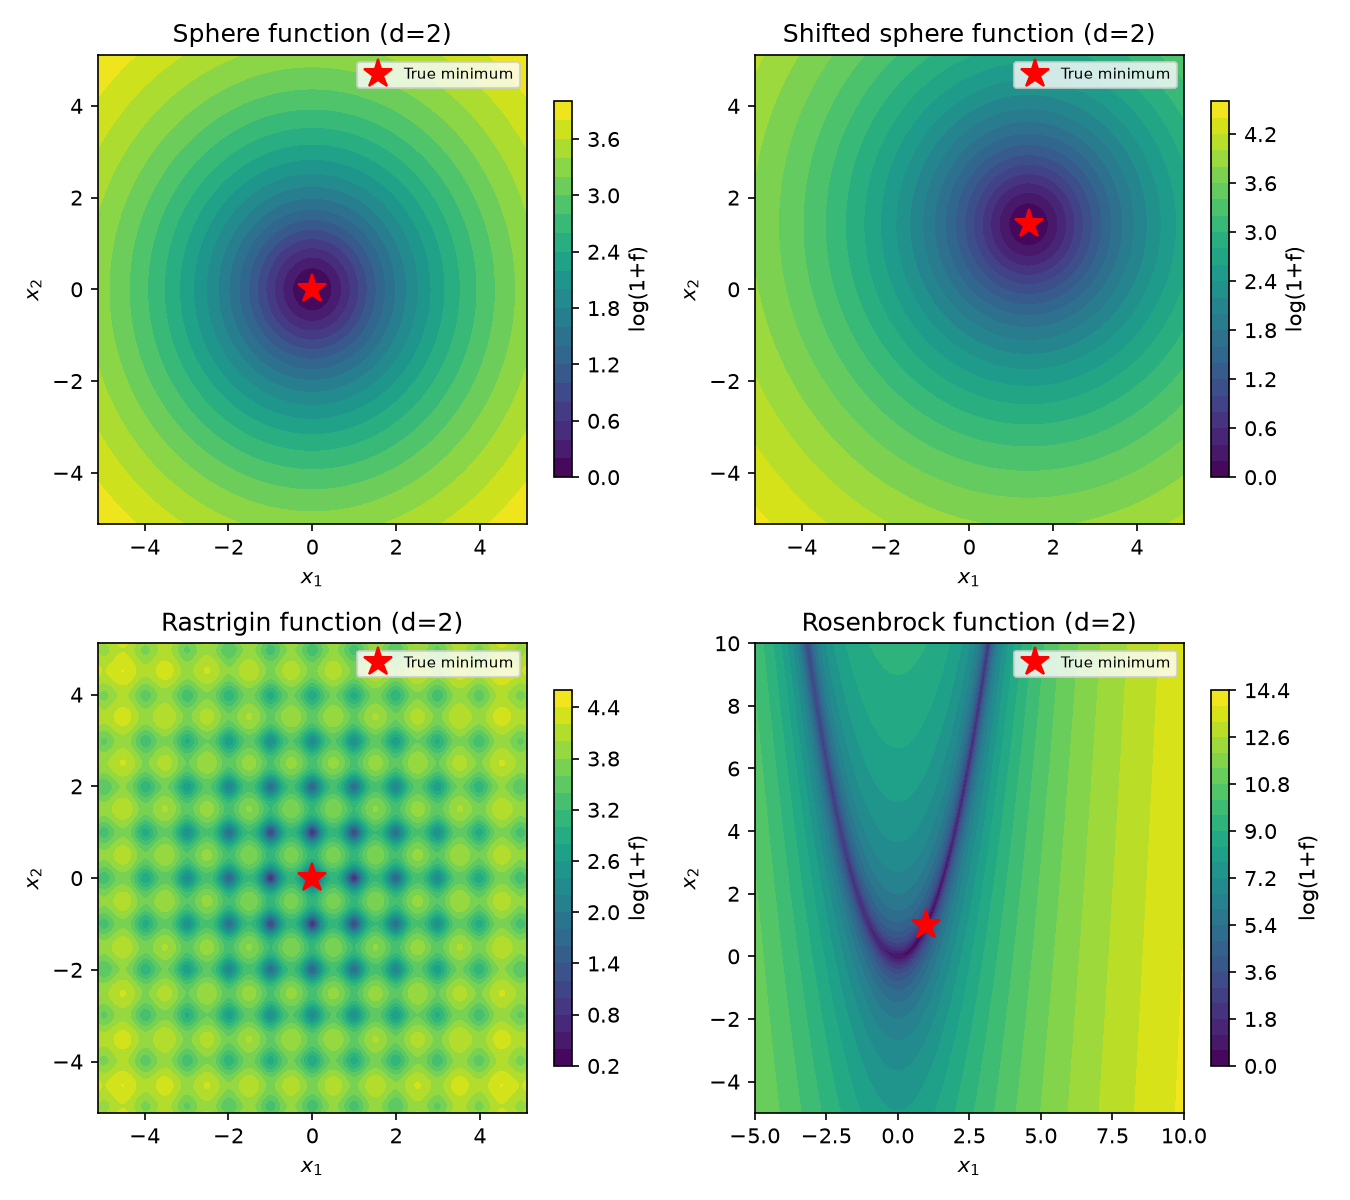
\includegraphics[width=0.48\textwidth]{../figures/benchmark_landscape_grid.png}
\caption{All four benchmark functions at $d = 2$, shown as contour maps on a log scale. The red star marks the true minimum in each case. Sphere and Shifted sphere are smooth bowls. Rastrigin is covered in regularly spaced local minima. Rosenbrock has a long, narrow, curved valley.}
\label{fig:landscapegrid}
\end{figure}

Figure~\ref{fig:landscapegrid} shows all four functions at $d = 2$, using a log scale, $\log(1+f(\mathbf{x}))$ is plotted instead of $f(\mathbf{x})$, since the raw values of the functions range from very small to very large depending on location, and the log scale makes the overall shape easier to see. The original project assignment on which this paper was built required that of the Sphere and the Shifted sphere to be tested at $d = 2, 5, 10$, and Rastrigin and Rosenbrock, both of which required $d > 1$ to be tested at $d = 2,5$. In this paper, all four functions are tested in all three dimensions, $d = 2, 5, 10$, for a total of twelve test cases, ensuring a complete and consistent evaluation of the algorithm. For each function and each dimension, the Grey Wolf Optimizer is run 20 separate times, each time starting from a different random population of wolves, with larger populations and more iterations used for the harder problems. Running the algorithm 20 separate times checks two things simultaneously, whether it actually finds a solution close to the known correct solution, and how stable it is, whether it produces similar results across repeated runs. The best result from the 20 runs is reported as the final solution for each test, along with the mean and spread of all 20 results.

\subsection{The SEIR disease model}

\begin{figure}[H]
\centering
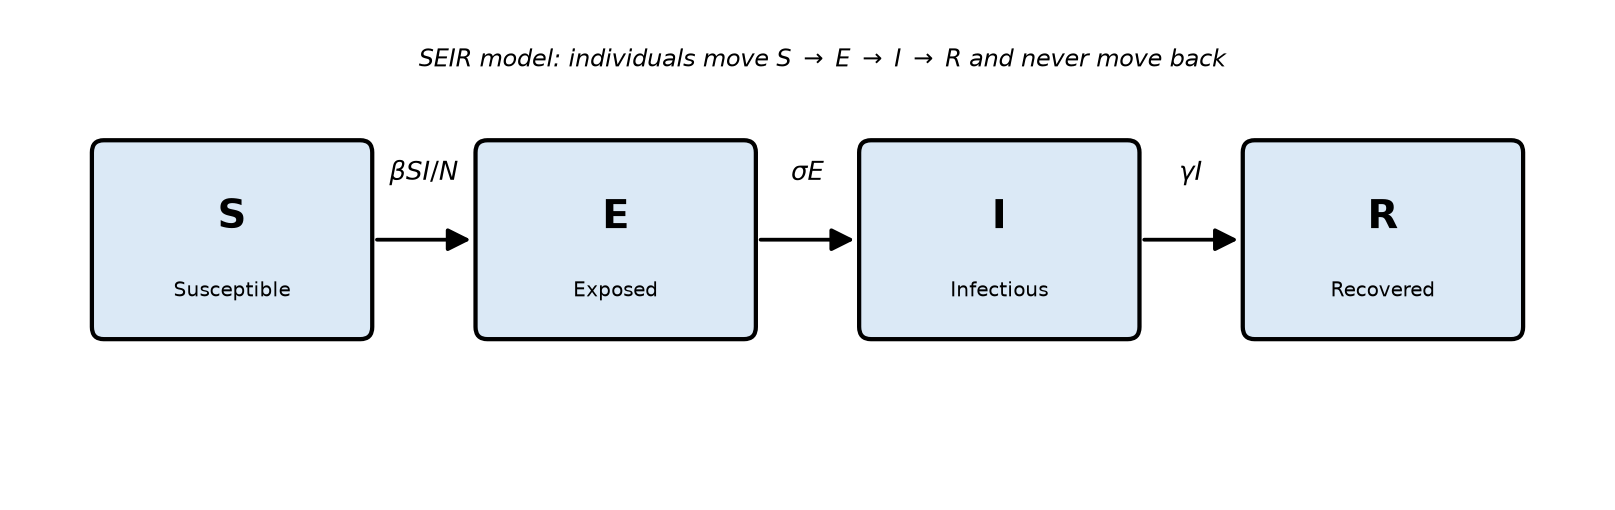
\includegraphics[width=0.48\textwidth]{../figures/seir_diagram.png}
\caption{The four compartments of the SEIR model, and the rate at which people move from one to the next.}
\label{fig:seirdiagram}
\end{figure}
Figure~\ref{fig:seirdiagram} shows the structure of the disease model. The Ghanaian population is divided into four compartments, and every person moves through them in one direction only, never backward. $S(t)$ is the number of people susceptible at time $t$ (measured in days since the start of the outbreak), that is, people who have not yet caught the disease and can still become infected. $E(t)$ is the number of people exposed, who have been infected but are not yet infectious, because they are still in the early silent stage of infection. $I(t)$ is the number of infectious individuals who can transmit the disease to others. $R(t)$ is the number of recovered individuals who cannot catch or spread the disease. At every moment, $S(t)+E(t)+I(t)+R(t)=N$, where $N$ is the total population. The model is as follows

\begin{align}
\frac{dS}{dt} &= -\beta \frac{S I}{N},\\
\frac{dE}{dt} &= \beta \frac{S I}{N} - \sigma E, \\
\frac{dI}{dt} &= \sigma E - \gamma I,\\
\frac{dR}{dt} &= \gamma I
\end{align}
Here, $dS/dt$ means the rate at which $S$ changes over time $t$, and the same pattern applies to the other compartments. $\beta$ is the transmission rate that controls the speed with which the disease spreads from an infectious person to a susceptible one; a larger $\beta$ means faster spread. $\sigma$ is the rate at which an exposed individual becomes infectious, equal to 1 divided by the average number of days spent in the exposed stage (the incubation period). $\gamma$ is the recovery rate, equal to 1 divided by the average number of days that an individual remains infectious before recovering.

\subsection{The basic reproduction number}

The basic reproduction number, $R_0$, is the average number of new infections caused by an infectious person, in a fully susceptible population. It is the most informative number produced by this model. $R_0 > 1$ means that an outbreak keeps growing, while $R_0 < 1$ means that it shrinks and eventually stops. For this model, $R_0 = \beta/\gamma$. This can be derived formally using the next-generation matrix method of \cite{vandendriessche2002}, the standard approach for computing $R_0$ in compartmental models. The method separates the equations for the infected compartments, $E$ and $I$, into new infections entering the system (matrix $\mathcal{F}$) and all other kind of movements(matrix $\mathcal{V}$), both evaluated near the start of an outbreak where $S \approx N$. Ordering the compartments as
$(E,I)$

\begin{equation}
\mathcal{F} = \begin{pmatrix} 0 & \beta \\ 0 & 0 \end{pmatrix}, 
\end{equation}


\begin{equation}
\mathcal{V} = \begin{pmatrix} \sigma & 0 \\ -\sigma & \gamma \end{pmatrix} 
\end{equation}

$R_0$ is defined as the largest eigenvalue of $\mathcal{F}\mathcal{V}^{-1}$.
\iffalse
where an eigenvalue is a number that tells us how much a matrix stretches things in a given direction, and the largest one here measures how fast new infections can multiply.
\fi
Computing this gives:

\begin{equation}
\mathcal{V}^{-1} = \begin{pmatrix} 1/\sigma & 0 \\ 1/\gamma & 1/\gamma \end{pmatrix},
\end{equation}

\begin{equation}
\mathcal{F}\mathcal{V}^{-1} = \begin{pmatrix} \beta/\gamma & \beta/\gamma \\ 0 & 0 \end{pmatrix}
\end{equation}
which has eigenvalues $\beta/\gamma$ and $0$, giving the following

\begin{equation}
R_0 = \frac{\beta}{\gamma}.
\end{equation}

This matches the simpler intuitive argument, an infectious person remains infectious for $1/\gamma$ days on average, and infects $\beta$ new people per day while infectious, giving $\beta \times (1/\gamma) = \beta/\gamma$ total infections. The formal method above is the general one that still works for more complicated models.

\subsection{Why the reporting fraction and starting condition trade off}
\label{sec:growthrate}

Section~\ref{sec:unconstrained-results} shows, by repeated testing, that the reporting fraction and the initial number of exposed individuals cannot be determined uniquely from the case data alone. This can be shown analytically. Near the start of an outbreak, while it is still small, $S(t) \approx N$, so the equations for $E$ and $I$ no longer depend on $S$ or $R$

\begin{equation}
\frac{dE}{dt} \approx \beta I - \sigma E, 
\end{equation}

\begin{equation}
\frac{dI}{dt} = \sigma E - \gamma I.
\end{equation}
Looking for a solution where both compartments grow at the same exponential rate $r$, written $E(t) = E^\ast e^{rt}$ and $I(t) = I^\ast e^{rt}$, and substituting gives

\begin{equation}
(r+\sigma)E^\ast = \beta I^\ast, 
\end{equation}

\begin{equation}
(r+\gamma)I^\ast = \sigma E^\ast.
\end{equation}
Combining these two equations gives the well known relationship between an outbreak's growth rate and its parameters
\cite{wallinga2007}

\begin{equation}
(r+\sigma)(r+\gamma) = \beta \sigma.
\label{eq:growth}
\end{equation}
Equation~\eqref{eq:growth} fixes the growth rate $r$, which can be measured directly from the rate at which real cases rise, as a function of $\beta$ alone, since $\sigma$ and $\gamma$ are already known. This is why $\beta$ is easy to identify from the data regardless of the other unknown parameters. However, the number of cases reported during this early growth phase is approximately

\begin{equation}
C(t) \approx \rho \kappa E_0 \left(e^{rt} - 1\right)
\label{eq:earlyC}
\end{equation}
where $\rho$ is the reporting fraction (the proportion of true infections that are detected and reported), $E_0$ is the initial number of exposed individuals, and $\kappa$ is a constant depending only on $\beta$, $\sigma$, $\gamma$, not on $\rho$ or $E_0$. Equation \eqref{eq:earlyC} shows directly that the first reported cases depend on $\rho$ and $E_0$ only through their product $\rho \times E_0$, not separately. This is exactly the trade off found numerically in Section~\ref{sec:unconstrained-results}. The only way to break this tie is to bring in external information not contained in the case count data; such as fixing $\rho$ using independent seroprevalence evidence, as done in Section~\ref{sec:constrained-results}. 

\subsection{Fixed parameters and numerical method}

$\sigma$ and $\gamma$ describe the biology of the disease, instead of how it spread Ghana specifically, so they were fixed using values measured in previous medical research. $\sigma$ was set at $1/5.1$ per day, the average COVID-19 incubation period reported by \cite{lauer2020}. $\gamma$ was set at $1/7$ per day, a commonly used average infectious period. $N$ was set at 31,887,809, the World Bank's 2020 population estimate for Ghana \cite{worldbank2020}. The cumulative reported cases predicted by the model were calculated as $C(t) = \rho \cdot (I(t) + R(t))$, because $I(t) + R(t)$ is the total number of individuals who have entered the infectious compartment by day $t$, with everyone leaving $I$ moving to $R$ and staying there. The four equations were solved numerically using the fourth order Runge Kutta method (RK4), which takes small steps forward in time, using four evaluations of the rate of change at each step for an accurate result. Writing the whole system as $\dot{\mathbf{y}} = f(\mathbf{y})$ for the state vector $\mathbf{y} = (S,E,I,R)$, an RK4 step of size $h$ computes:

\begin{align}
\mathbf{k}_1 &= f(\mathbf{y}_n), \\
\mathbf{k}_2 &= f\!\left(\mathbf{y}_n + \tfrac{h}{2}\mathbf{k}_1\right), \\
\mathbf{k}_3 &= f\!\left(\mathbf{y}_n + \tfrac{h}{2}\mathbf{k}_2\right), \\
\mathbf{k}_4 &= f\!\left(\mathbf{y}_n + h\mathbf{k}_3\right), \\ \mathbf{y}_{n+1} &= \mathbf{y}_n + \frac{h} {6}\left(\mathbf{k}_1 + 2\mathbf{k}_2 + 2\mathbf{k}_3 + \mathbf{k}_4\right)
\end{align}
using a step size of $h = 1/4$ day. This fixed step size method was used over adaptive solvers because during model fitting the system needs to be solved tens of thousands of times, and this method is fast while still accurate enough for a smoothly changing system like this one.

\subsection{Letting the transmission rate change once}

Because a single constant transmission rate cannot explain an outbreak that slows long before susceptible depletion becomes significant, the model was extended to allow a change in transmission rate. The rate switches from $\beta_1$ to $\beta_2$, on a change day $t_c$, which is also estimated by the optimizer

\begin{equation}
\beta(t) = \begin{cases} \beta_1, & t \leq t_c \\ \beta_2, & t > t_c \end{cases}
\end{equation}
This produces two effective reproduction numbers, $R_0^{(1)} = \beta_1/\gamma$ before the change and $R_0^{(2)} = \beta_2/\gamma$, using the same formula derived above, which applies at any moment in time.

\subsection{Fitting procedure}

The Grey Wolf Optimizer minimizes the log scale sum of squared error between the model and the real data

\begin{equation}
\text{SSE} = \sum_t \Big(\log(1{+}C_{\text{model}}(t)) - \log(1{+}C_{\text{data}}(t))\Big)^2
\end{equation}

The logarithm is used because Ghana's case counts range from single digits to tens of thousands, and a plain squared error measure would be dominated almost entirely by the largest values near the end of the time window. Three fitting procedures were carried out: An unconstrained fit lets $\beta$, $\rho$, and $E_0$ all free. A constrained fit fixes $\rho$ from external evidence and leaves $\beta$ and $E_0$ free. A two phase fit extends the constrained model to let the transmission rate vary once. In each case, the fitting process was repeated independently many times (20, 20 and 10 runs), each starting from a different random wolf population, to test whether the fitted parameters remained consistent.

\section{Results}
\subsection{Testing the algorithm on standard problems}
\begin{table}[H]
\caption{Testing the Grey Wolf Optimizer on four standard math
problems at three sizes each. Each row summarizes 20 separate runs. The true correct answer is 0 in every case.}
\label{tab:benchmark}
\small
\begin{tabular}{lrrr}
\toprule
Function ($d$) & Best & Mean & Spread \\
\midrule
Sphere (2) & $1.4{\times}10^{-71}$ & $2.9{\times}10^{-50}$ & $1.2{\times}10^{-49}$ \\
Sphere (5) & $4.4{\times}10^{-39}$ & $4.8{\times}10^{-32}$ & $1.8{\times}10^{-31}$ \\
Sphere (10) & $7.2{\times}10^{-36}$ & $7.4{\times}10^{-32}$ & $1.9{\times}10^{-31}$ \\
Shifted sphere (2) & $7.3{\times}10^{-8}$ & $1.9{\times}10^{-6}$ & $1.7{\times}10^{-6}$ \\
Shifted sphere (5) & $1.5{\times}10^{-5}$ & $4.8{\times}10^{-5}$ & $3.0{\times}10^{-5}$ \\
Shifted sphere (10) & $6.2{\times}10^{-5}$ & $1.3{\times}10^{-4}$ & $3.2{\times}10^{-5}$ \\
Rastrigin (2) & $0.0$ & $0.0$ & $0.0$ \\
Rastrigin (5) & $0.0$ & $5.0{\times}10^{-2}$ & $2.2{\times}10^{-1}$ \\
Rastrigin (10) & $0.0$ & $2.48$ & $2.57$ \\
Rosenbrock (2) & $3.2{\times}10^{-8}$ & $1.7{\times}10^{-6}$ & $1.5{\times}10^{-6}$ \\
Rosenbrock (5) & $4.7{\times}10^{-1}$ & $1.23$ & $4.7{\times}10^{-1}$ \\
Rosenbrock (10) & $5.17$ & $5.93$ & $5.6{\times}10^{-1}$ \\
\bottomrule
\end{tabular}
\end{table}

Table~\ref{tab:benchmark} shows the results of all 12 test cases. The Grey Wolf Optimizer reliably found the known correct solution, or a value extremely close to it, in every case. Sphere and Rastrigin were solved almost exactly even at the largest size tested. Rosenbrock, whose narrow valley makes fine convergence difficult, was solved less precisely as the size grew, matching its known difficulty, and confirming the algorithm behaves as expected before being trusted on real data.

\begin{figure}[H]
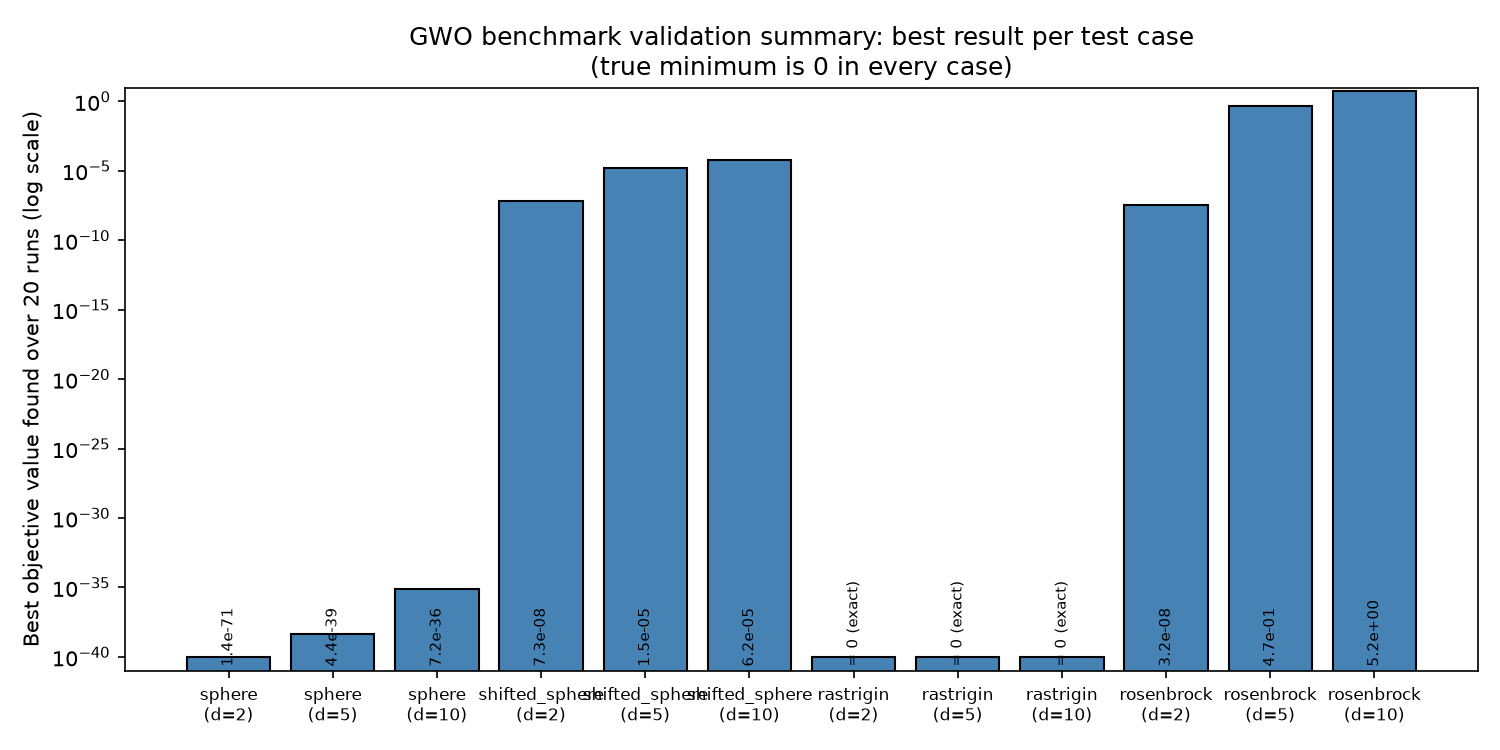
\includegraphics[width=0.48\textwidth]{../figures/benchmark_summary.png}
\caption{Best answer found (log scale) across all 12 test cases. The true answer is 0 in every case.}
\label{fig:benchmarksummary}
\end{figure}

\begin{figure}[H]
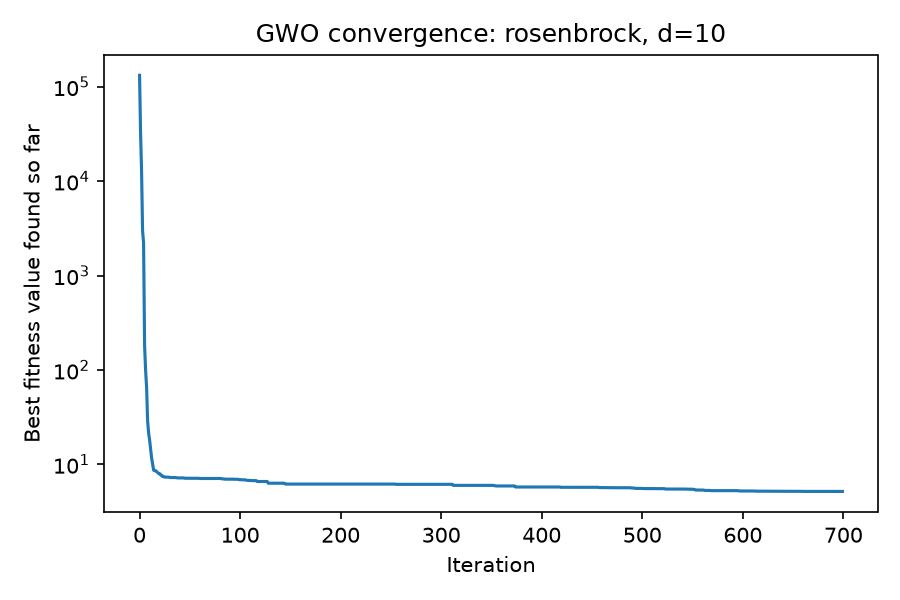
\includegraphics[width=0.48\textwidth]{../figures/convergence_rosenbrock_d10.png}
\caption{How the best answer found improved during the search, for the hardest test case, Rosenbrock at $d=10$, best of 20 runs.}
\label{fig:convrosen}
\end{figure}
\vspace{-20pt}

\subsection{Unconstrained fit reveals a real identifiability problem}
\label{sec:unconstrained-results}

Across 20 independent runs of the unconstrained model, $\beta$
consistently settled near 0.19 in most runs (13 of 20), but $\rho$ and $E_0$ spread widely among runs, reaching an almost identical fit (within 1 percent of the best SSE, 119.42). $\rho$ ranged from 0.060 to 0.078 while $E_0$ ranged from 2,397 up to the search limit of 3,000. A smaller group of runs (8 of 20) settled on a clearly different solution instead, with $\beta \approx 0.49$ and $\rho \approx 0.001$, reaching a noticeably worse fit (SSE near 150) that still looked reasonable at first glance.

\begin{figure}[H]
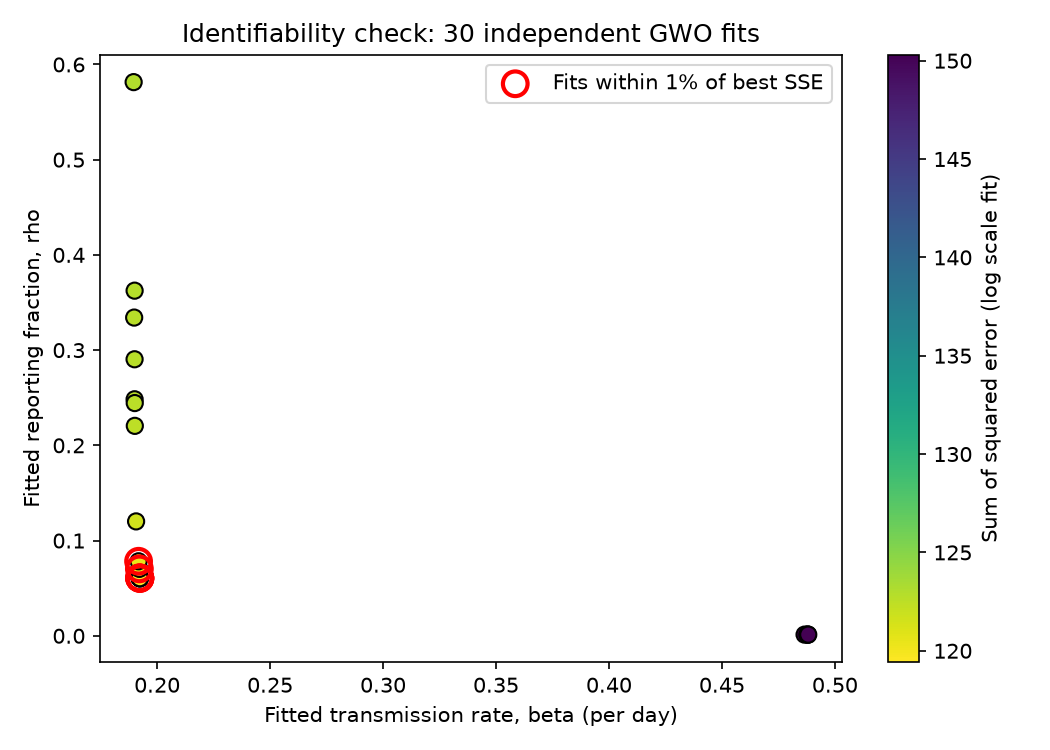
\includegraphics[width=0.48\textwidth]{../figures/identifiability_beta_rho.png}
\caption{Fitted $\beta$ against fitted $\rho$, across 20 separate runs of the unconstrained model. Points circled in red are within 1\% of the best fit. Good fits cluster on one $\beta$ but spread widely in $\rho$.}
\label{fig:identplot}
\end{figure}

This is a direct demonstration of the practical identification problem described in Section II-C and matches exactly what Equation~\eqref{eq:growth} and Equation~\eqref{eq:earlyC} estimate. Many different combinations of $\rho$ and $E_0$ that keep their product the same can reproduce almost the same early growth curve, so case count data alone cannot tell them apart.

\subsection{Fixing the problem with outside evidence}
\label{sec:constrained-results}

$\rho$ was fixed at 0.05, informed by a nationally representative Ghanaian seroprevalence survey finding a cumulative exposure of 67.1\% by December 2021 against a much smaller confirmed case total \cite{owusudonkor2023}, and by international estimates of COVID-19 under detection in March 2020 ranging from about 2.4\% to 100\% in 84 countries \cite{russell2020}. With $\rho$ fixed, $\beta$ converged to 0.1921 in every one of the 20 separate runs (spread of only 0.0001), giving $R_0 \approx 1.34$.

\begin{figure}[H]
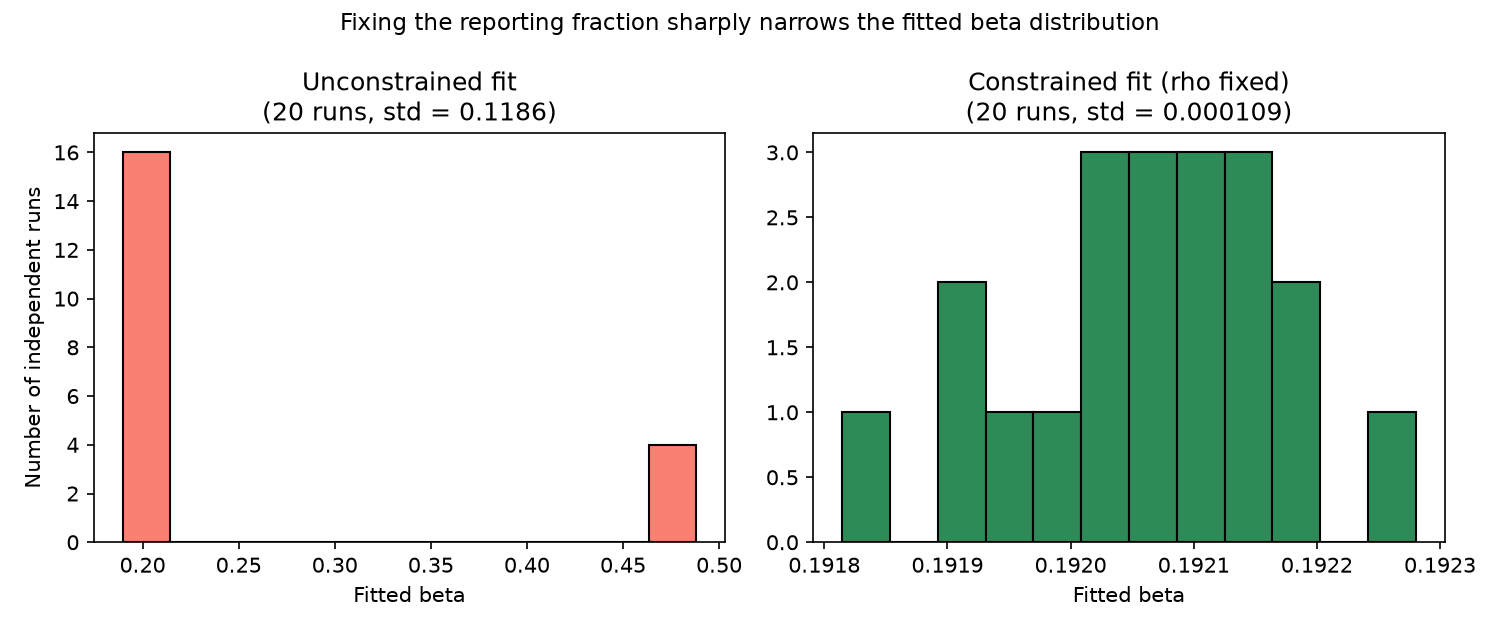
\includegraphics[width=0.48\textwidth]{../figures/beta_identifiability_comparison.png}
\caption{Fitted $\beta$ spread across 20 restarts, before (left) and after (right) fixing $\rho$. The spread shrinks from about 0.12 to about 0.0001.}
\label{fig:betacomparison}
\end{figure}

Figure~\ref{fig:betacomparison} shows this improvement directly, the standard deviation of the fitted $\beta$ shrinks by about three orders of magnitude once $\rho$ is fixed using external evidence, not more computing power.

\begin{figure}[H]
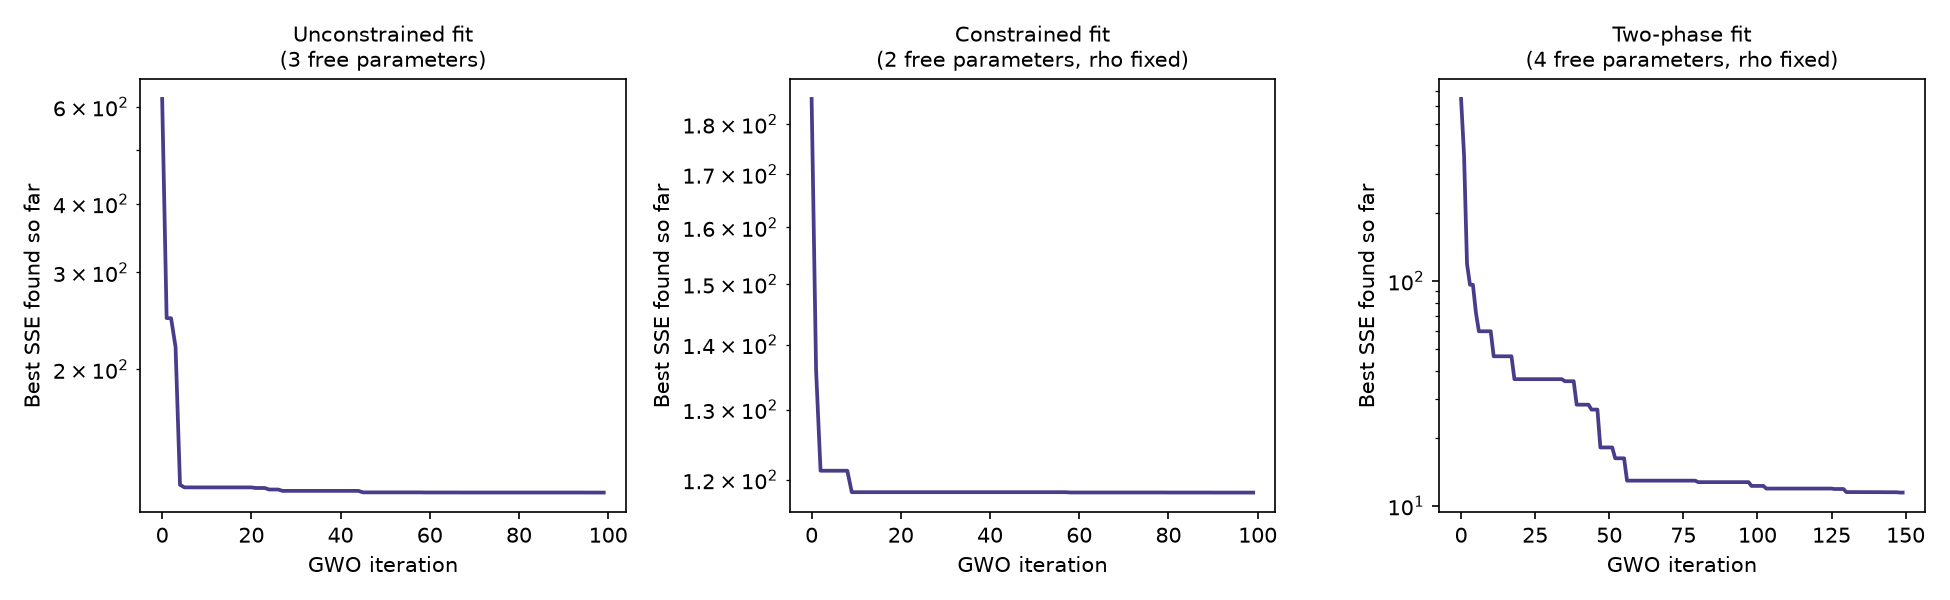
\includegraphics[width=0.48\textwidth]{../figures/gwo_convergence_seir_all.png}
\caption{How the best fit found improved during the search, for the best run of each of the three fitting stages. Every search levels off well before the end, confirming enough steps were used.}
\label{fig:seirconv}
\end{figure}

\subsection{A model with a changing rate captures the whole wave}
\label{sec:two-phase-results}
The constrained single rate model fits the early growth well but overshoots badly after day 150, because susceptible depletion alone cannot explain a slowdown reached at less than 3\% of the population. Allowing the transmission rate to vary once a day, as the optimizer found, fixed this. Nine out of ten independent runs converged to $\beta_1 \approx 0.345$ ($R_0 \approx 2.41$) before day 50 of the outbreak, changing to $\beta_2 \approx 0.155$ ($R_0 \approx 1.09$) afterward, reducing the log scale SSE from about 118 to about 11.5 and reaching an $R^2$ of 0.934 on the original scale. The one remaining run settled on a distinctly worse local minimum (SSE $\approx$ 36.5), a useful reminder that even a well behaved model can occasionally have the search settle on a worse local minimum by chance.

\begin{figure}[H]
\centering
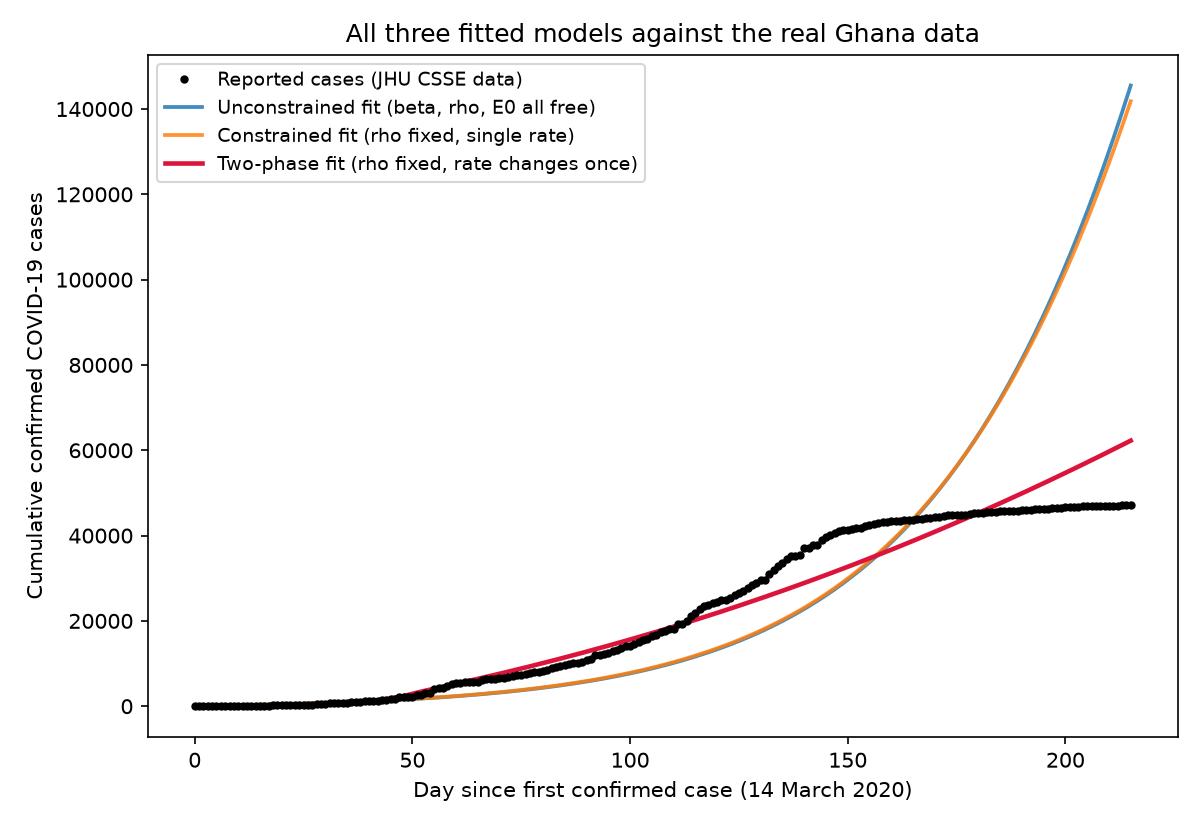
\includegraphics[width=0.48\textwidth]{../figures/model_comparison.png}
\caption{All three fitted models against the real data. The single rate models (blue, orange) drift away after day 150. The two phase model (red) tracks the real path throughout.}
\label{fig:modelcomp}
\end{figure}
\vspace{-38pt}

\begin{figure}[H]
\centering
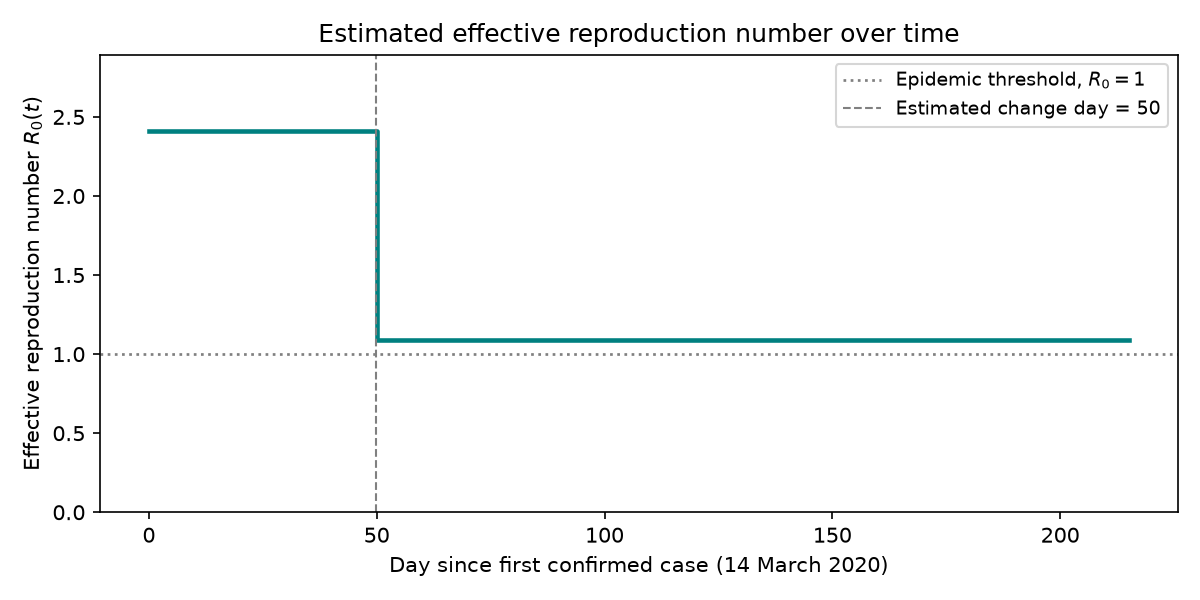
\includegraphics[width=0.48\textwidth]{../figures/r0_over_time.png}
\caption{Estimated effective reproduction number over time from the two phase fit, decreasing from approximately 2.41 to about 1.09 at the estimated change day.}
\label{fig:r0time}
\end{figure}

The estimated change day, around day 50, roughly early May 2020, falls shortly after Ghana's partial lockdown of Accra and Kumasi was lifted (20 April 2020) and its mask rule began (26 April 2020) \cite{kenu2020}, a consistent match to documented events, allowing for the natural delay between infection and a confirmed test result.

\begin{figure}[H]
\centering
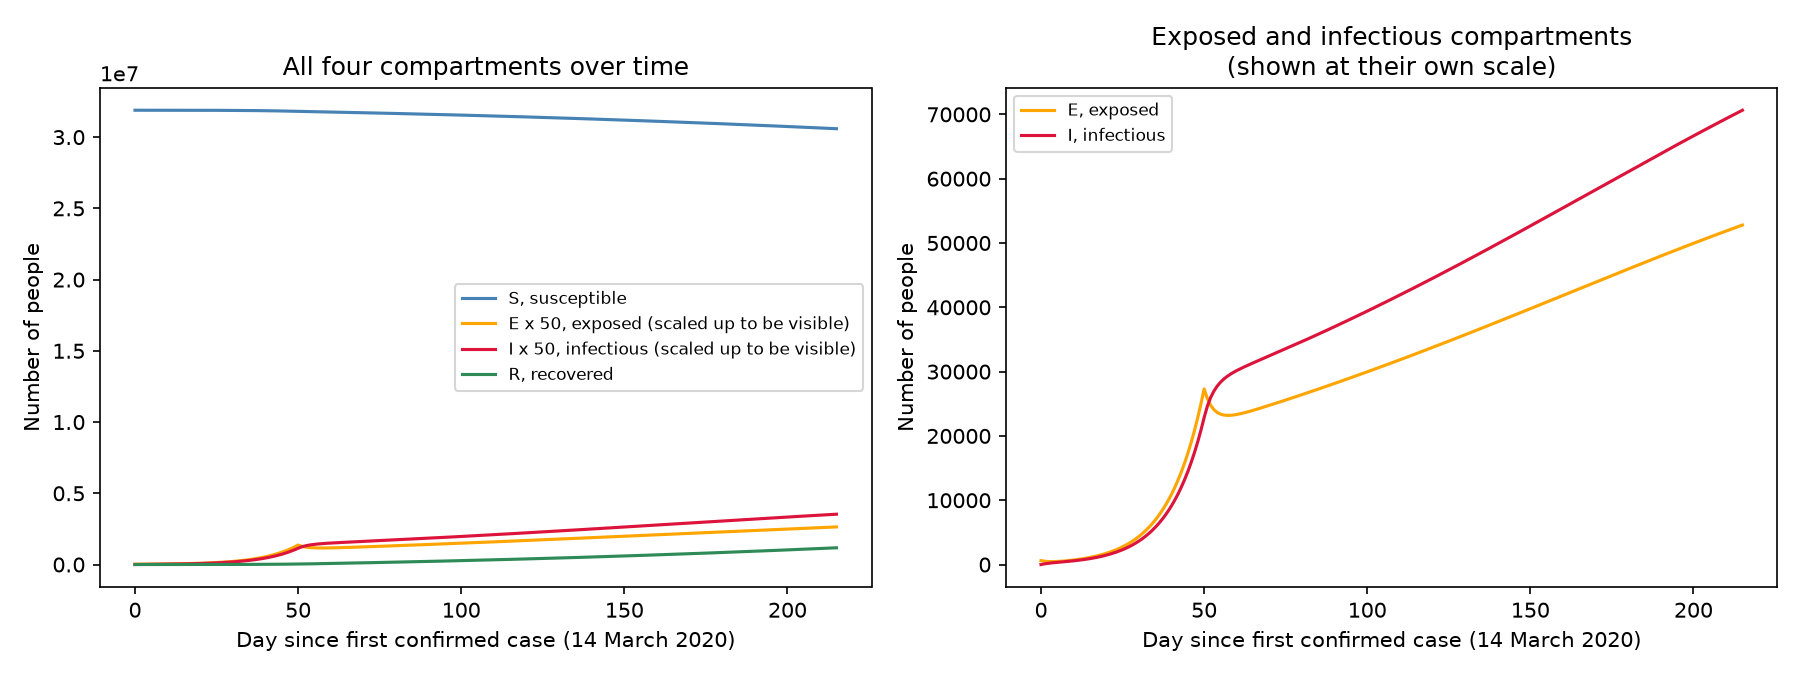
\includegraphics[width=0.48\textwidth]{../figures/seir_compartments_two_phase.png}
\caption{The full path of all four compartments for the best two phase fit. The susceptible compartment barely decreases, confirming that running out of susceptible people never explains the slow down.}
\label{fig:compartments}
\end{figure}

\begin{figure}[H]
\centering
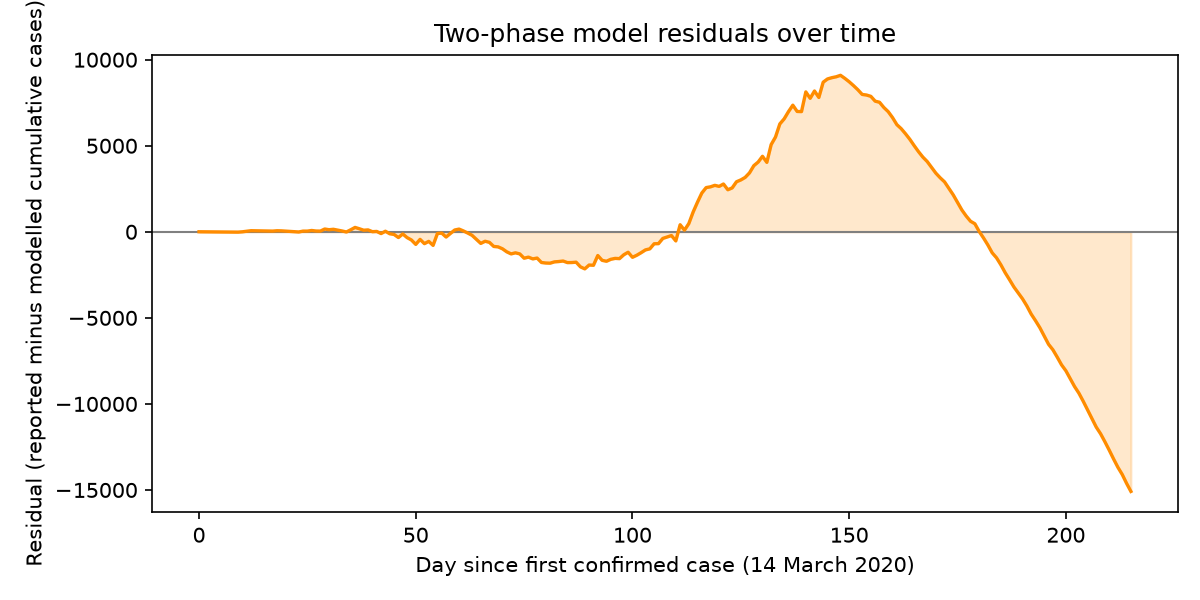
\includegraphics[width=0.48\textwidth]{../figures/two_phase_residuals.png}
\caption{Two phase model residuals over time. The smooth curving pattern, rather than random noise, suggests the real transmission rate changed more gradually than this model's single sharp switch.}
\label{fig:residuals}
\end{figure}

\section{Discussion}

\begin{table}[H]
\centering
\caption{Summary of all three fitting stages. SSE is the log-scale sum of squared error used during fitting. $R^2$ is computed on the original, non-logged scale, for the two-phase model only, since this is the only stage that fits the data well enough for this measure to be meaningful.}
\label{tab:summary}
\small
\begin{tabular}{lccc}
\toprule
& Unconstrained & Constrained & Two-phase \\
\midrule
Free parameters & 3 & 2 & 4 \\
Independent runs & 20 & 20 & 10 \\
Best SSE & 119.42 & 118.26 & 11.47 \\
$\beta$ (or $\beta_1$) & 0.192 & 0.1921 & 0.345 \\
$\beta$ spread (std) & 0.119 & 0.0001 & n/a \\
$\rho$ & free (0.06-0.08) & fixed, 0.05 & fixed, 0.05 \\
$R_0$ (or $R_0^{(1)}$) & 1.33 & 1.34 & 2.41 \\
$R_0^{(2)}$ & -- & -- & 1.09 \\
R squared & n/a & poor fit & 0.934 \\
\bottomrule
\end{tabular}
\end{table}

Table~\ref{tab:summary} brings together the key parameters of all three fitting stages side by side. Moving from left to right across the table shows the numerical story of this paper. The unconstrained fit produced a low spread in $\beta$ but a wide, unreliable spread in $\rho$. Fixing $\rho$ in the constrained fit collapses the spread in $\beta$ by about three orders of magnitude, but the single fixed transmission rate cannot yet explain the entire outbreak. If the constrained model were evaluated across the entire duration of 216-days using the same $R^2$ measure used for the two phase model, its sharp mismatch would be immediately visible. Only the two phase model, with the additional structure of a changing transmission rate, achieves a genuinely good fit across the full duration. This study aimed to do two major things. First, we test a metaheuristic search algorithm on standard benchmark problems with known solutions, and second, we use that algorithm to fit a real disease model to real data while being explicit about whether the resulting parameter estimates could be trusted. The first part established confidence that the search algorithm works correctly. The second part produced something more valuable, even though it was not simple at first. Fitting the model without any constraints did not yield a clean, reliable solution. Instead, it revealed a real identifiability problem between the reporting fraction and the number of individuals exposed initially, matching a well known difficulty in fitting disease models to case count data. Demonstrating this directly, using many independent search runs rather than a single fitted curve, provides a more honest and more informative way to report such results.

Fixing this identifiability problem needed external information, real evidence of Ghana's reporting fraction, not additional computation. Once this outside information was incorporated, the transmission rate was precisely and consistently identified. This matters because the transmission rate and the reproduction number derived from it are usually the quantity on which public health decisions are based. The two phase extension shows a related point. A model that fits well is not by default a model that is correctly specified. The single rate model fits the early outbreak well and could easily appear successful if only early data were examined, but it diverges sharply once the real outbreak's growth slows. Only by fitting the full time window does this weakness become clear.

\section{Limitations}

Despite the contributions of this work, several limitations should be acknowledged. 

\begin{itemize}
    \item The reporting fraction $\rho = 0.05$ used in Section~\ref{sec:constrained-results} thereafter is an informed estimate based on real evidence, but it is not a value measured directly for Ghana's first wave in 2020. The used seroprevalence study was carried out in 2021. A useful next step would be to treat $\rho$ as uncertain within a reasonable range, for example, using a Bayesian approach, rather than fixing it at a single value.

    \item  The SEIR model is intentionally simple. It does not include age structure, does not represent the fact that the Ghana outbreak was concentrated in a few major cities, and does not model changes in testing availability over time.

    \item The two-phase transmission rate model is a simple substitute for what was probably a more gradual and more complex real change in transmission. The smooth curvature in the residuals after day 150 (Figure~\ref{fig:residuals}) suggests that a model with multiple change points, or a smoothly varying transmission rate, would fit even better, at the cost of additional parameters and more identifiability challenges.

    \item This work models only Ghana's first wave. Extending the approach to later waves, which involved new variants of the virus and vaccination, would require additional model components.

    \item The identifiability analysis presented here, though shown both numerically and analytically, applies only to the specific three-and four-parameter models used. A larger model with more unconstrained parameters would require a different identifiability assessment, which could reveal different or additional trade-offs.
\end{itemize}  

\section{Future work}

The approach applied in this work, fitting a mechanistic disease model to real surveillance data using a metaheuristic search algorithm, then directly testing and, where needed, resolving identifiability challenges using external evidence, is general and not tied to COVID-19 or Ghana specifically. Several future directions follow from it.

One direction could be to apply the same approach to tuberculosis
transmission, a disease where nonidentifiability and the connection between social and economic conditions and disease spread are already active areas of research. Tuberculosis case-notification data, similar in structure to the COVID-19 case counts used here, are publicly available for many countries through the World Health Organization. A future extension could build a compartment model of tuberculosis
spread in a specific setting and study how parameter identifiability depends on the surveillance data available, connecting population-level case counts to core social determinants of disease.

A second direction follows from the identifiability analysis. Section~\ref{sec:growthrate} used a simple linear analysis of the model's early growth phase to show exactly why two parameters traded off. This kind of manual analysis becomes much difficult as a model grows larger and more realistic, for instance, with age structure, multiple locations, or several disease strains.
Developing more general, automated methods for detecting and quantifying non-identifiability in large models, buildingon the observation that repeated  metaheuristic searches from different starting points can already serve as a practical diagnostic tool.

A third direction could extend the modelling toward viral infections with more complex immune dynamics, beyond the relatively simple SEIR structure utilized in this study. It is well established that retroviruses that establish long-lasting infections involve ongoing interactions between the virus and the immune system, and fitting such within-host models to real patient data is likely to raise identifiability questions possibly as challenging as those studied in this paper.

A fourth direction concerns the spatial dimension this work does not address. The SEIR model used in this work assumed a well-mixed population, but real outbreaks, including Ghana's, are not spatially homogeneous. Extending the compartmental structure to a reaction-diffusion formulation, a potential application in which this study's approach could inform.

\iffalse
since within host viral load and immune marker data typically offers fewer, noisier observations than a population-level case count time series. The approach demonstrated here, testing a chosen optimizer on known problems first, then using it to fit a real model while directly checking whether the fitted
parameters can be trusted, extends naturally to this setting, moving from population level disease counts toward within host viral dynamics and immune response modelling more broadly.
\fi


More broadly, real-world surveillance data is almost always an incomplete and imperfect view onto the true process being studied, and a model that fits such data well is not, on its own, evidence that its parameters mean what we think they mean. Building routine identifiability checks into how disease models are fit and reported, across the wide range of settings in public health modelling, viral dynamics modelling and immune responses, is a direction this paper hopes to encourage.

\section{Conclusion}

This paper built and tested the Grey Wolf Optimizer on twelve standard benchmark problems with known solutions, and then used it to fit an SEIR disease model to real COVID-19 case data from Ghana's first pandemic wave. Fitting the model without constraints showed a clear identifiability problem between the disease's true reporting fraction and the initial number of exposed individuals, which was resolved using external evidence from Ghanaian seroprevalence studies and international under-reporting estimates. Once resolved, the transmission rate became precisely and
consistently identified across many independent search runs. Because a single, constant transmission rate could not reproduce the full outbreak curve, the model was extended to allow one change in transmission over time, greatly improving the fit and producing results consistent with Ghana's documented public-health response in 2020. The source code is available \href{https://github.com/Frank-Anokye/gwo-seir-identifiability}{here}.

\bibliographystyle{IEEEtran}
\bibliography{references}

\iffalse
\section*{Reproducibility}

All code, data, figures, and result tables used in this paper are openly available on the accompanying GitHub repository. The code folder holds the Grey Wolf Optimizer implementation, the benchmark functions, the SEIR model in both its single-rate and two-phase forms, and all of the fitting and figure generating scripts. The data folder holds the raw, unedited case count data downloaded from JHU CSSE, alongside the smaller, processed file actually used for fitting. The results folder contains every numerical result table referenced in this paper, and the figures folder contains every figure shown here at full resolution. Every script resolves its own file locations automatically using its own file path, rather than depending on the folder it happens to be run from, so that the entire pipeline can be run again, from scratch, on any computer, without changing a single line of code. Every fitting run in this paper used a fixed, recorded random
seed, so every number reported here can be reproduced exactly.
\fi
\end{document}
